% -*- coding: utf-8 -*-
% \documentclass[journal]{IEEEtran}
\documentclass[titlepage, twocolumn, a4paper, 10pt]{article}
\usepackage{parskip}
\usepackage[english]{babel}
\usepackage[utf8]{inputenc}
\usepackage{verbatim}
\usepackage{fancyhdr}
\usepackage{graphicx}
\usepackage{url}
\usepackage{varioref}

%%%%%%%%%%%%%%%%
% Column spacing
% \setlength{\columnsep}{7mm}
\renewcommand{\sfdefault}{phv}
\renewcommand{\rmdefault}{ptm}
\renewcommand{\ttdefault}{pcr}

\hyphenpenalty=750
% If we didn't adjust the interword spacing, 2200 might be better.
% The TeX default is 1000
\hbadness=1350
% IEEE does not use extra spacing after punctuation
\frenchspacing

% V1.7 increase this a tad to discourage equation breaks
\binoppenalty=1000 % default 700
\relpenalty=800     % default 500


% margin note stuff
\marginparsep      10pt
\marginparwidth    20pt
\marginparpush     25pt


% if things get too close, go ahead and let them touch
\lineskip            0pt
\normallineskip      0pt
\lineskiplimit       0pt
\normallineskiplimit 0pt

\topmargin    -49.0pt
\headheight   12pt
\headsep      0.25in

\textheight       58pc  % 9.63in, 696pt
\columnsep         1pc
\textwidth        42pc   % 2 x 21pc + 1pc = 43pc

% the default side margins are equal
\oddsidemargin        0.680in
\evensidemargin       0.680in
% compensate for LaTeX's 1in offset
\addtolength{\oddsidemargin}{-1in}
\addtolength{\evensidemargin}{-1in}
\topmargin        -0.25in
% we retain the reserved, but unused space for headers
\addtolength{\topmargin}{-\headheight}
\addtolength{\topmargin}{-\headsep}

%%%%%%%%%%%%%%%%


\usepackage[pdfborder={0 0 0 0}]{hyperref}

% Include pdf with multiple pages ex \includepdf[pages=-, nup=2x2]{filename.pdf}
\usepackage[final]{pdfpages}

% Place figures where they should be use [H]
\usepackage{float}

% Float for text
\floatstyle{ruled}
\newfloat{code}{!htb}{lop}
\floatname{code}{CodeSnippet}

% vars
\def\title{UmuMe, a RESTful service}
\def\preTitle{Project report}
\def\kurs{Service-Oriented Architectures, HT-09}

\def\namn{Anton Johansson}
\def\mail{dit06ajn@cs.umu.se}

\def\namnTva{Jonny Strömberg}
\def\mailTva{dit06jsg@cs.umu.se}


\def\pathtocode{\url{dit06ajn~/edu/soa/umume}}
\def\handledareEtt{P-O Östberg, p-o+soa@cs.umu.se}

\def\inst{Computer Science}
\def\dokumentTyp{Report}

\begin{document}
\begin{titlepage}
  \thispagestyle{empty}
  \begin{small}
    \begin{tabular}{@{}p{\textwidth}@{}}
      UMEÅ UNIVERSITY \hfill \today \\
      Department of \inst \\
      \dokumentTyp \\
    \end{tabular}
  \end{small}
  \vspace{10mm}
  \begin{center}
    \LARGE{\preTitle} \\
    \huge{\textbf{\kurs}} \\
    \vspace{10mm}
    \LARGE{\title} \\
    \vspace{15mm}
    \begin{large}
      \namn, \mail \\
      \namnTva, \mailTva\\
      Code-path: \texttt{\pathtocode}\\
      \vspace{10mm}
    \end{large}
    \vfill
    \large{\textbf{Supervisors}}\\
    \mbox{\large{\handledareEtt}}\\
  \end{center}
\end{titlepage}

\newpage
\mbox{}
\vspace{70mm}
\begin{center}
  % Dedication goes here
\end{center}
\thispagestyle{empty}
\newpage

\pagestyle{fancy}
\rhead{\today}
\lhead{\footnotesize{\namn, \mail\\\namnTva, \mailTva}}
\chead{}
\lfoot{}
\cfoot{}
\rfoot{}

\cleardoublepage
\newpage
\onecolumn
\tableofcontents
\twocolumn
\cleardoublepage

\fancyfoot[LE,RO]{\thepage}
\pagenumbering{arabic}

\section{Introduction}\label{sec:intro}
% Beskriv med egna ord vad uppgiften gick ut på. Är det någonting som
% varit oklart och ni gjort egna tolkningar så beskriv dessa.
This report describes the work done designing and implementing a RESTful web service providing information about employees and students at Umeå university. For this web service a client web site is done to highlight possible uses of the web service.

The main idea with the web service is to combine information from the
existing information about every employee/student with a possibility
for persons to add information about themselves. This added extra
information can for example be a brief description, visiting location
and usernames for other web services such as
Twitter\footnote{\url{http://twitter.com/}} to enable mashup
implementations.

The web service will hereby be referred to as \textit{Umume-rest}, a
combination of \textit{Umu} as in Umeå university and \textit{me}
because it provides a service for students and employees to add
information about themselves. The client web site will be referred to
as \textit{Umume-website}. All students and employees at Umeå
university are potential users of our service, they will hereafter be
refereed to as simply users.

These implementations are done with the programming language
\textit{Java}\footnote{\url{http://java.sun.com/}}, uses the framework
\textit{Spring
  Framework}\footnote{\url{http://www.springframework.org/}} for the
web site and
\textit{Jersey}\footnote{\url{https://jersey.dev.java.net/}} for the
RESTful Web service.

The original project specification for the work described in this
report is in Appendix \ref{app:ps}.

\section{Problem analysis}\label{sec:problem-analysis}
% As this project emphasizes analysis and investigation of a loosely
% specified problem, include any assumptions you made during the
% analysis phase in your report. Also discuss problems encountered and
% alternative solutions considered in the analysis. The report should
% also discuss to what extent the requirement list is fulfilled, as
% well as to which extent you could adhere to the the project plan.
Since the \textit{Umume-rest} is created to enable third party
developers to access information and create their own web service, it
was decided to make the web service RESTful instead of using the SOAP
protocol. This decision was made because in a RESTful web service
every resource have a unique identifier easily accessible with a
simple HTTP GET method call. For example the information about a
person could be fetched by pointing a web browser to
\url{http://example.com/users/aonjon04}. This for example enables the
development of simple AJAX Javascript clients that use our service,
this is demonstrated and described in Section \ref{sec:web-search}.

The web service \textit{Umume-rest} builds mainly on two existing
services provided by Umeå university, a Lightweight Directory Access
Protocol directory service (LDAP) and a Central Authentication Service
(CAS).

\subsection{LDAP}\label{sec:ldap}
All preexisting informations about users is fetched from an LDAP
directory service provided by the university at
\url{ldap://ldap.umu.se}. This directory service contains information
about every student and employee. Every user is uniquely identified by
a 8 character string such as "aonjon04". With every unique user comes
extra information such as faculty membership, email addresses, phone
numbers and so on.

An initial idea was to use address information about every user and
map this information to a longitude and latitude to plot the users
positions an a map, for example by using Google Maps
API\footnote{\url{http://code.google.com/apis/maps/}}. This idea was
however discarded since the structure of location information from
LDAP was inconsistent between different users and faculties.

The most important service provided by LDAP used by
\textit{Umume-rest} is the possibility to search for first- and
surnames to retrieve their unique CAS-username. This username is used
to authenticate users, see the Section \ref{sec:cas}.

\subsection{Central Authentication Serive}\label{sec:cas}
Every employee and student at Umeå university can get a CAS-user and
password by physically visiting a reception and identifying
themselves. This CAS-user enables access to different services around
campus, for example accessing the wireless network, scientific
articles and checking results from finished courses. More information
about CAS can be found at
\url{http://www.it.umu.se/vara-tjanster/centralt-anvandarnamn/cas/}
(in Swedish).

The CAS used by \textit{Umume-rest} is located at
\url{https://cas.umu.se/} and is used by \textit{Umume-rest} to
authenticate requests to add or change information about your own
user. This means that no extra username or password is required for
users of \textit{Umume-rest} and that users only can edit their own
information.

% TODO: Discuss single point of failure?

\section{Compilation and deployment}\label{sec:compile}
All files needed to use set up the web service are located at:\\
\texttt{\pathtocode/umume-rest}\\
and the files for the web site are at:\\
\texttt{\pathtocode/umume-website}

Commands in following section will require the software tool
\textit{Apache Ant}\footnote{http://ant.apache.org/}. More details
about what happens using when \textit{ant} in this project is found in
the \textit{build.xml} files\footnote{http://ant.apache.org/manual/using.html}.

This project has been deployed within \textit{Apache Tomcat
  6.0.20}\footnote{http://tomcat.apache.org/} as Servlet container but
any Java Servlet container should do.

\subsection{Umume-rest}
This section explains how to compile and deploy the
\textit{Umume-rest} web service.

To deploy \textit{umume-rest} issue the following command:\\
\begin{footnotesize}
  \verb!salt:./umume-rest> ant deploy!
\end{footnotesize}\\
This will create a directory \verb!target! if it does not already
exists and compile and move compiled files and configuration files to
that directory. Then a war file is generated and moved to the Servlet
container specified by \textit{deploy.dir} in
\texttt{conf/build.properties}.

The root-directory for class-files when using \textit{Umume-rest} is
compiled to \textit{target/classes/}, while the root-directory for
test-code is compile to \textit{target/test-classes/}.

To create portable \textit{war}-file of the compiled sources issue the
following command:\\
\begin{footnotesize}
  \verb!salt:./umume-rest> ant war!
\end{footnotesize}\\
This will create \textit{umume-rest.war} which can be deployed within
any Java servlet container.

Third party libraries that \textit{Umume-rest} depend upon are
specified int the file \texttt{ivy.xml}, issuing \textit{ant resolve}
will download and install all those libraries in the \texttt{lib} folder.

\subsection{Umume-website}
This section explains how to understand, compile and deploy the
\textit{umume-website} web page.

To deploy \textit{umume-website} issue the following command:\\
\begin{footnotesize}
  \verb!salt:./umume-website> ant deploy!
\end{footnotesize}\\
This will create a directory \verb!war/WEB-INF/classes! if it does not
already exists and compile/move source-code and configuration files to
that directory. Then the catalog is copied to the the pre-defined
Servlet container specified by \textit{deploy.dir} in
\texttt{conf/build.properties}.

To create and deploy a portable \textit{war}-file from the compiled
sources issue the following command:\\
\begin{footnotesize}
  \verb!salt:./umume-rest> ant deploywar!
\end{footnotesize}\\
This will create and deploy \textit{umume.war}.

\section{Usage}\label{sec:usage}
% Förklara var programmet och källkoden ligger samt hur man kompilerar,
% startar och använder det. Förklara även översiktligt vad som händer
% när man använder de olika kommandona. Det räcker alltså inte att
% skriva "man skriver 'ant' för att kompilera", utan det måste även ingå
% en liten förklaring om vad som egentligen händer när man kör ant och
% varför det fungerar. Använd Internet eller litteratur för att själva
% ta reda på den information ni tycker känns relevant, dels för
% rapportens skull och dels för er egen. Kom ihåg att skriva tydliga
% (vetenskapliga) referenser!

This description explains how to communicate with the web sercive and
how to navigate on the web site.

\subsection{Umume-rest}
An instance of the \textit{Umume-rest} should be running with
resources at base URI \url{http://mega.cs.umu.se:8080/umume-rest/}
from \today\ and some time further. Secure access for PUT updates are
available at \url{https://mega.cs.umu.se:8443/umume-rest/}.

There are two different resources in the service. Both allows GET
requests and and one of them also allows authorised users to add or
change information with PUT requests.
\begin{itemize}
\item GET \verb!/users/{uid}! returns information about a user in
  either \textit{application/xml} or \textit{application/json}
  depending on which the user requested with an Accept HTTP header.
\item PUT
  \texttt{/users/\{uid\}?ticket=\{CAS-ticket\}\\\&service=\{service-url\}}
  updates information about the specified user if the request contains
  a CAS-ticket and the service-URI at which the ticket is granted. The
  format of the request is \textit{application/xml}. For more
  information see CodeSnippet \ref{code:put-request}.
\item GET \verb!/search/{searchString}! returns a list of users
  matching the provided search string in either
  \textit{application/xml}, \textit{application/json} or
  \textit{application/javascript} depending on which the user
  requested.
\end{itemize}

\begin{code}
  \begin{footnotesize}
\begin{verbatim}
<person>
    <description>My own description</description>
    <latitude>23.1234</latitude>
    <longitude>63.1234</longitude>
    <twitterName>MyTwitterName</twitterName>
</person>
\end{verbatim}
  \end{footnotesize}
  \caption{PUT request example}\label{code:put-request}
\end{code}

\subsection{Umume-website}

The images in Figure
\ref{fig:images/startpage}-\vref{fig:images/edited-user} describes how
to navigate through the \textit{Umume-website} to view and update
information about yourself. You should be able to follow this scenario
at \url{http://piko.cs.umu.se:8080/umume/} which should be available
some time from \today.
\newpage
\begin{figure}[H]
  \centering
  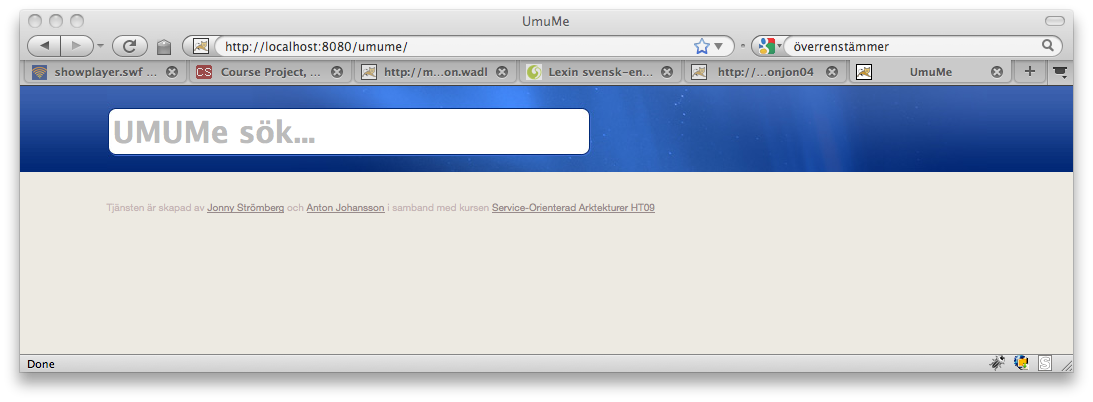
\includegraphics[width=3.3in]{images/pic1.png}
  \caption{Start page.}
  \label{fig:images/startpage}
\end{figure}

\begin{figure}[H]
  \centering
  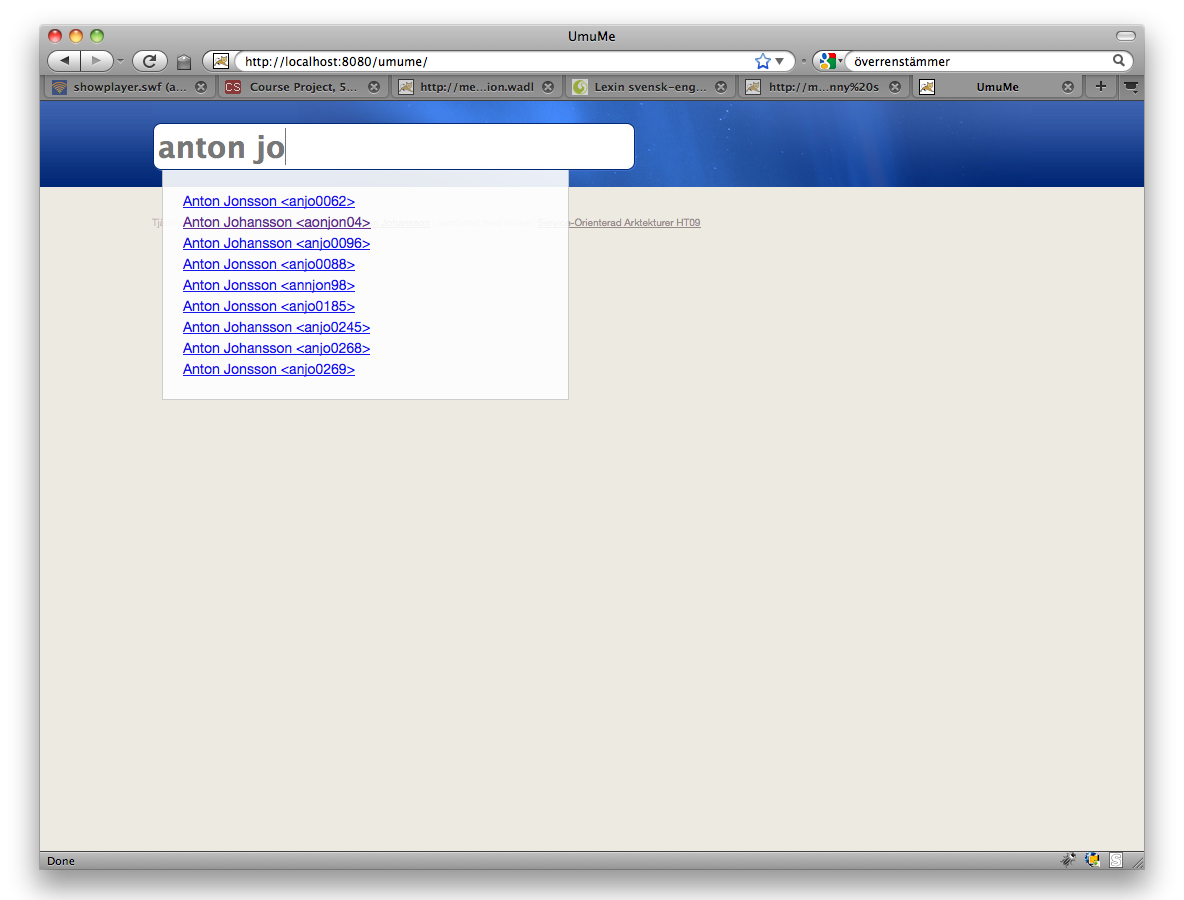
\includegraphics[width=3.3in]{images/pic2.png}
  \caption{Search for yourself.}
  \label{fig:images/search}
\end{figure}

\begin{figure}[H]
  \centering
  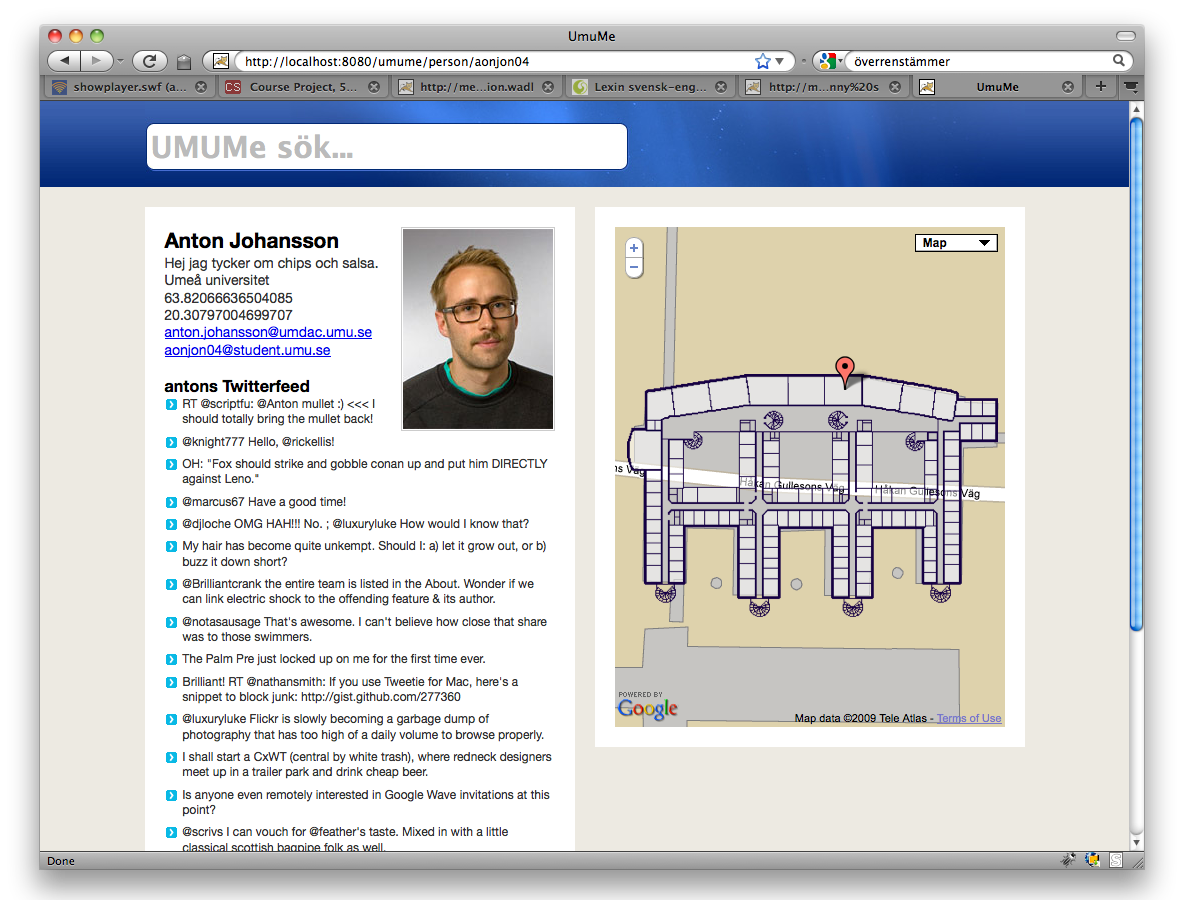
\includegraphics[width=3.3in]{images/pic3.png}
  \caption{User profile, eventually with Twitter-feed and position at Google Maps.}
  \label{fig:images/person}
\end{figure}

\begin{figure}[H]
  \centering
  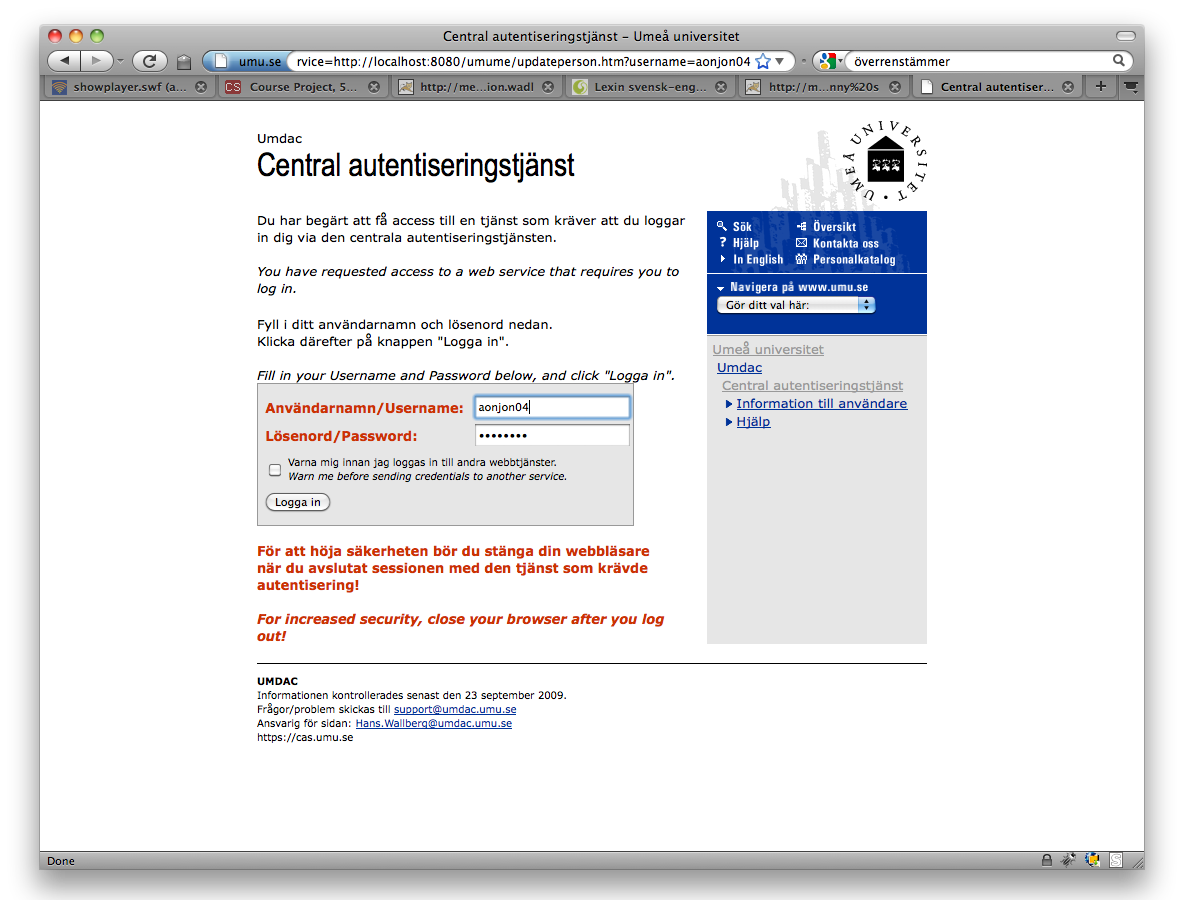
\includegraphics[width=3.3in]{images/pic4.png}
  \caption{Click on "uppdatera" at the bottom of the profile and then authorize CAS-user.}
  \label{fig:images/cas}
\end{figure}

\begin{figure}[H]
  \centering
  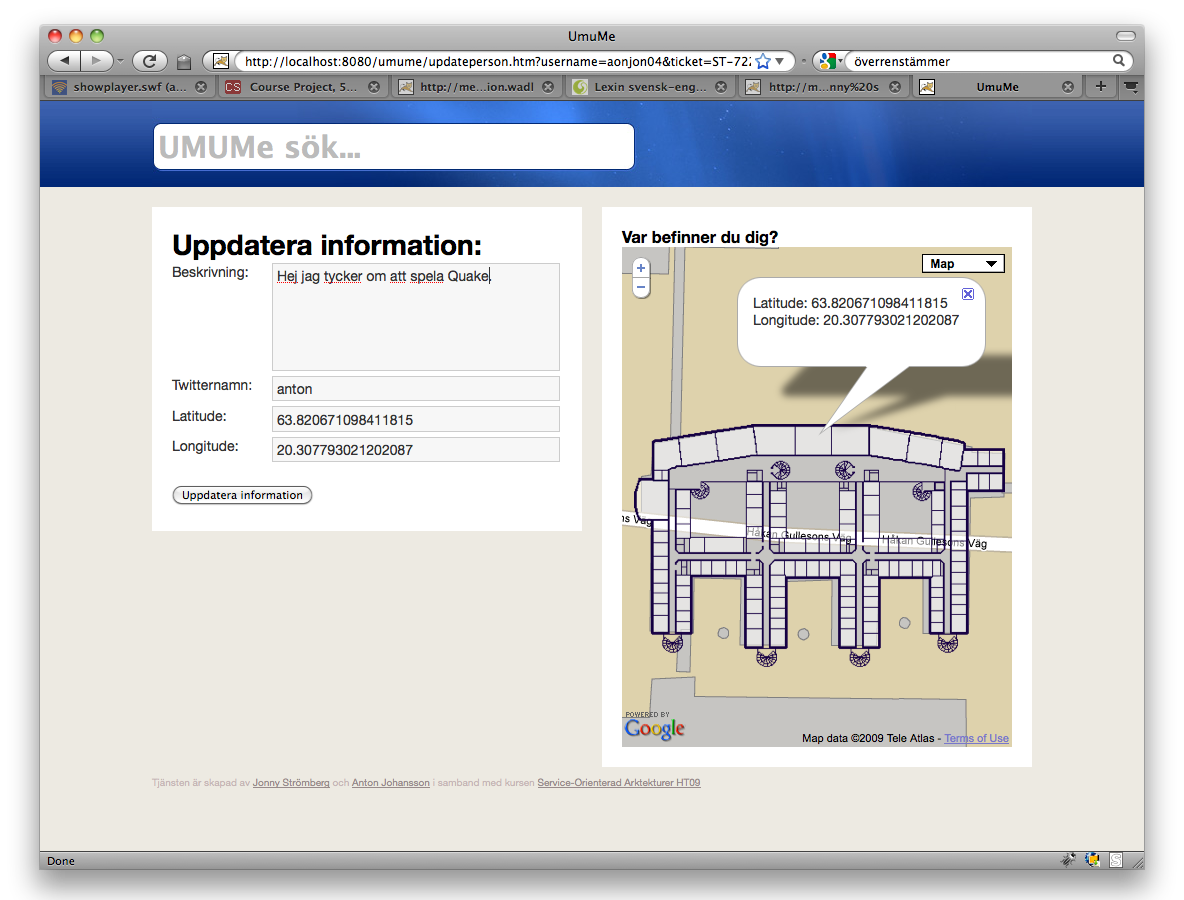
\includegraphics[width=3.3in]{images/pic5.png}
  \caption{Update user information in input boxes and click the map to
  update position.}
  \label{fig:images/edit}
\end{figure}

\begin{figure}[H]
  \centering
  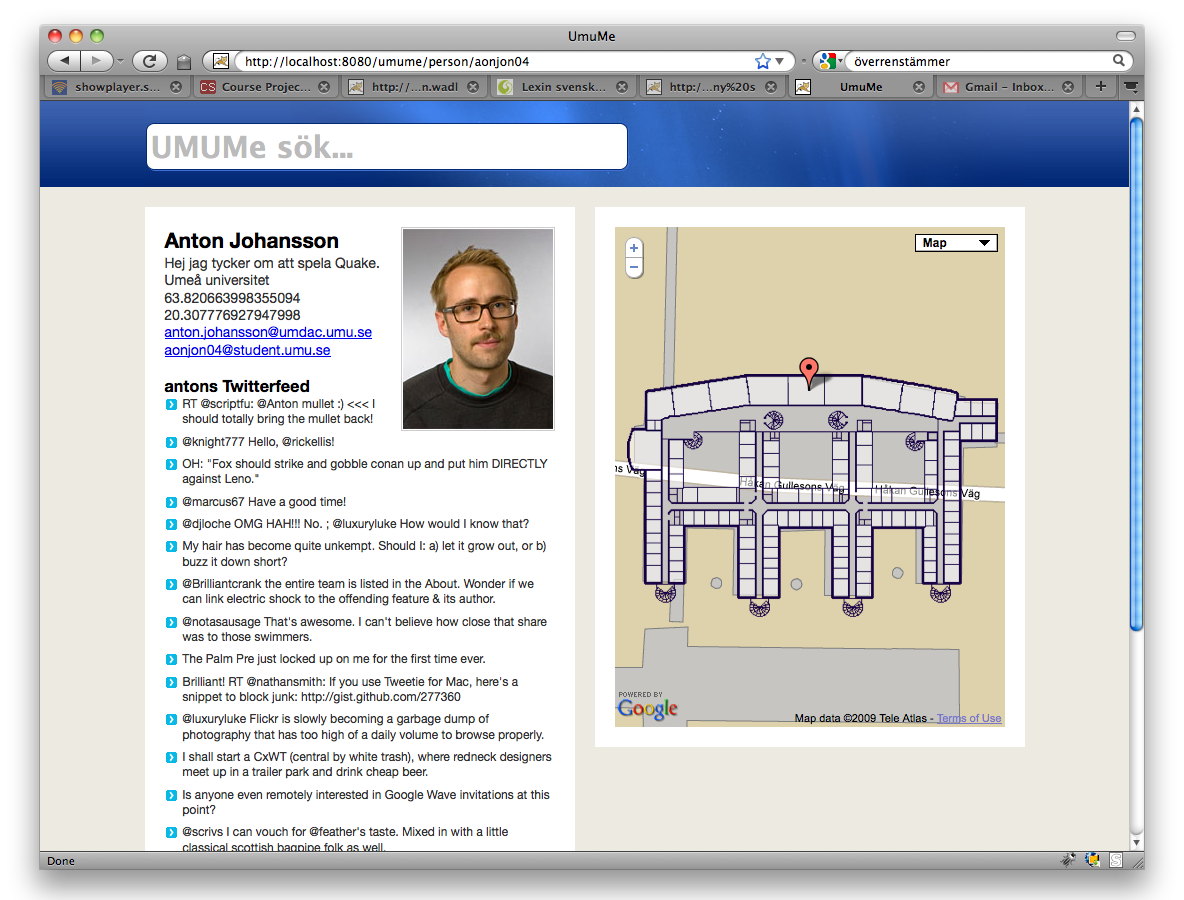
\includegraphics[width=3.3in]{images/pic6.png}
  \caption{See updated information (if the authorized CAS-user was the same as the updated profile.}
  \label{fig:images/edited-user}
\end{figure}
\newpage

\section{System description}\label{sec:system}
% Beskriv översiktligt hur programmet är uppbyggt och hur det löser
% problemet.


% \begin{figure*}[!h]
%   \centerline{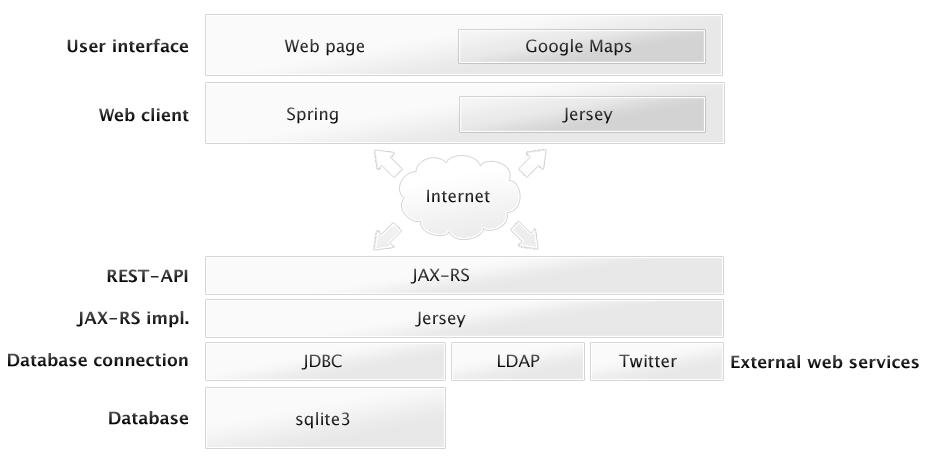
\includegraphics[width=140mm]{images/systemarchitecture.jpg}}
%   \caption{System design}
%   \label{fig:images/sysarch}
% \end{figure*}

The complete system described in this report consists of different
modules. The top part of this Figure \ref{fig:images/sysdes}
represents \textit{Umume-website} while the bottom part represents
\textit{Umume-rest}.

\begin{figure}[H]
  \centering
  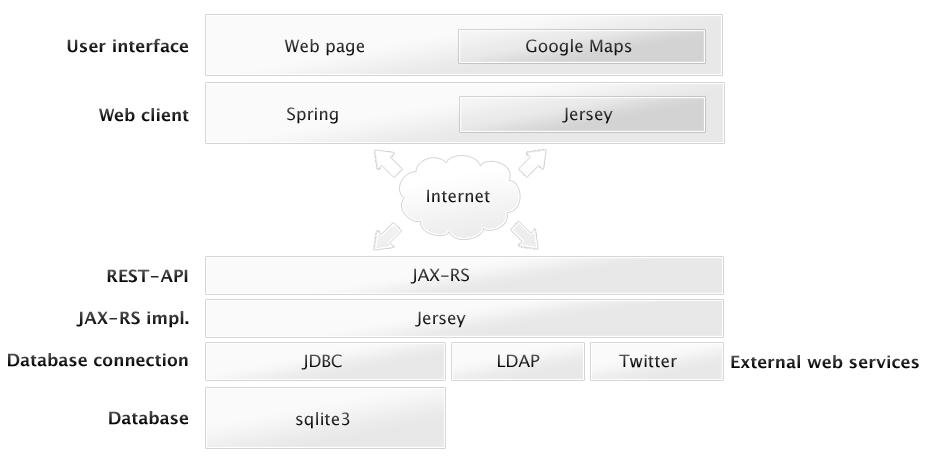
\includegraphics[width=3.3in]{images/systemarchitecture.jpg}
  \caption{System design}
  \label{fig:images/sysdes}
\end{figure}

\subsection{Umume-rest}\label{sec:umume-rest}
The RESTful web service uses the \textit{JAX-RS
  API}\footnote{\url{http://jcp.org/en/jsr/detail?id=311}} with the
\textit{Jersey}\footnote{https://jersey.dev.java.net/} implementation.
This enables resources to be defined within normal java classes by
merely adding annotations to specify at which path the resource is
available and what HTTP-methods the resource is accessable by. Se an
example in CodeSnippet \ref{code:jaxrs}. This is basically what is
used by \textit{Umume-rest} to provide resources describing users. A
java bean (\textit{PersonBean.java}) is used to represent users. This
bean is marshaled and unmarshal by
JAXB\footnote{\url{https://jaxb.dev.java.net/}} into different
mediatypes depending on what is requested. Our user resources can be
fetched as XML or JSON\footnote{\url{http://www.json.org/}} depending
on which HTTP Accept header is sent by the request. See example
responses from \textit{Umume-rest} in
Appendix~\ref{app:example-request-response}.

\begin{code}
  \begin{footnotesize}
\begin{verbatim}
// The resource is available at path /users/{uid}
@Path("/users/{uid}")
public class UsersResource {
    // The Java method will process HTTP GET requests
    @GET
    // It can return XML and JSON
    @Produces({"application/xml",
               "application/json"})
    public PersonBean getUserXML(
                   @PathParam("uid") String uid) {
        //...
        return person;
    }
}
\end{verbatim}
  \end{footnotesize}
  \caption{JAX-RS resource}\label{code:jaxrs}
\end{code}

The response from a request to a specific user is made up by first
getting all information about the user that LDAP provides, then
possible information from the persistance layer is added, lastly
various API calls are made to get extra information. In this case the
Twitter API is used to get Tweets. Figure~\ref{fig:images/personbean}
shows a summary of this communication.

\begin{figure}[!htb]
  \centering
  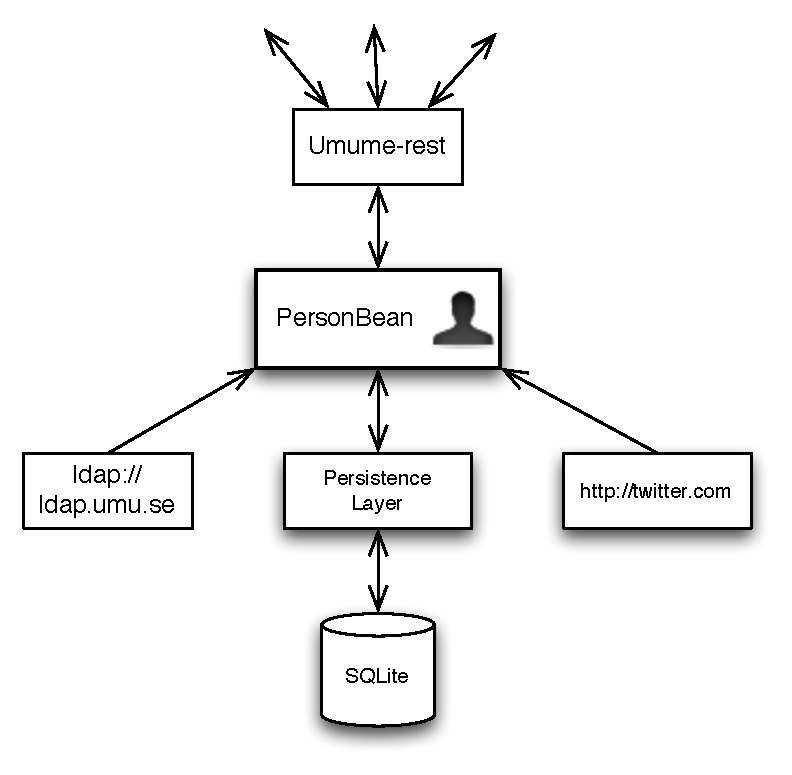
\includegraphics[width=3in]{images/personbean.pdf}
  \caption{Building a PersonBean}
  \label{fig:images/personbean}
\end{figure}


\subsubsection{Update user resource}\label{sec:updateuser}
To update a user resource a valid CAS user is required. The request is
made by a HTTP PUT request with new information about the referenced
user, see example implementation in CodeSnippet
\ref{code:updateResource}. This example consumes XML with updated
information about the user resource.

To validate whether the request is made from the user that the
resource is describing a CAS ticket is required as a query string.
This supplied ticket from CAS is then validated at
\url{https://cas.umu.se} using a
CAS-client\footnote{\url{http://www.jasig.org/cas}}. If the supplied
ticket is valid, a username can be extracted and if this username is
the same as the username of the resource to change it can be certain
that the request comes from the person who is represented by the
resource. Since a ticket is confidential information all this network
traffic is tunneled through a secure connection using the HTTPS
protocol. See Figure \ref{fig:images/auth} for an overview of this
communication.

\begin{code}
  \begin{footnotesize}
\begin{verbatim}
@PUT
@Consumes(MediaType.APPLICATION_XML)
public Response updateUser(
            @PathParam("uid") String uid,
            PersonBean pb,
            @QueryParam("ticket") String ticket,
            @QueryParam("service") String service) {
        // validate user, persist updated info
        return Response; //200 OK or errorcode
}
\end{verbatim}
  \end{footnotesize}
  \caption{Update resource}\label{code:updateResource}
\end{code}

\begin{figure}[!thb]
  \centering
  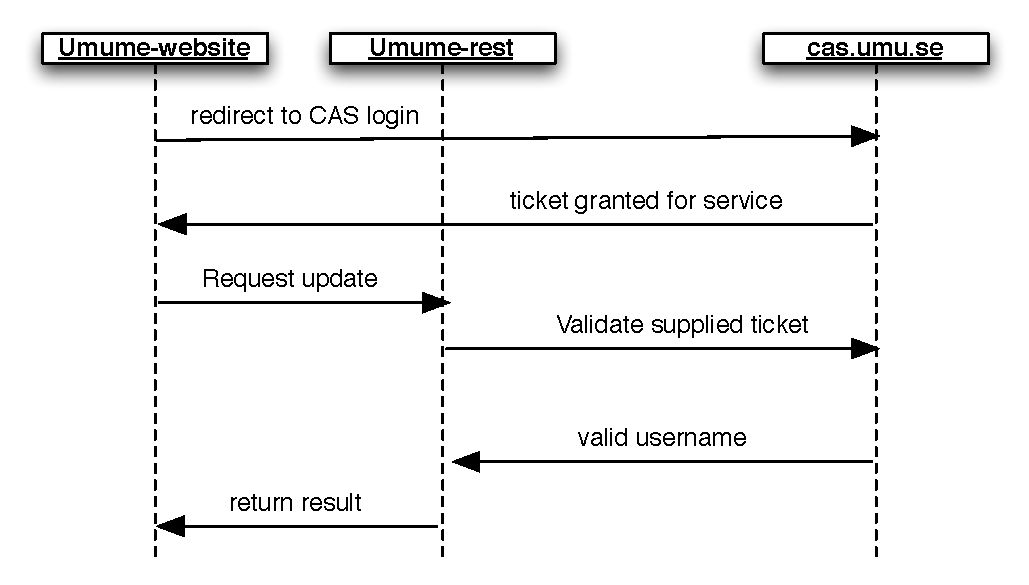
\includegraphics[width=3.3in]{images/auth.pdf}
  \caption{CAS authentication}
  \label{fig:images/auth}
\end{figure}

\subsubsection{Deployment: web.xml}
If \textit{Umume-rest} is compiled and archived into a WAR-file for
deployment, the file \texttt{web.xml} need to specify in which package
the resources are located, this can be seen in an excerpt from
\texttt{web.xml} in CodeSnippet \vref{code:webxml}. This file also
specifies that PUT requests on user resources need to be made with a
confidential transporting guarantee to make sure that CAS tickets are
confidential.

\begin{code}
  \begin{footnotesize}
\begin{verbatim}
<servlet>
   <servlet-name>UmumeREST</servlet-name>
   <servlet-class>
      com.sun.jersey.spi.\
      container.servlet.ServletContainer
   </servlet-class>
   <init-param>
      <param-name>
         com.sun.jersey.config.property.packages
      </param-name>
      <param-value>
         se.umu.cs.umume.rest.resources
      </param-value>
   </init-param>
</servlet>
\end{verbatim}
  \end{footnotesize}
  \caption{web.xml jersey resources}\label{code:webxml}
\end{code}

\subsubsection{Persistance layer}\label{sec:persistance}
To persist information received by PUT requests on user resources a
persistence layer using
JDBC\footnote{\url{http://java.sun.com/javase/technologies/database/}}
and SQLite\footnote{\url{http://www.sqlite.org/}} is used. In this
implementation this layer consists of a single Java class and a
portable SQLite database file.

When a request is made to update a user resource the new information
is inserted or updated into this specified database. Prepared
statements are used to prevent SQL injection attacks.

If a user resource has persisted data this is appended to response
returned. Most information returned is not stored in the Persistence
layer though. This implementation stores information about longitude,
latitude, a Twitter username and a description for the user.

The reason for choosing SQLite is that it made development easy since
the database file could be deployed and managed along with the rest of
the project. No separate processes needs to be started to get things
working. This also has some disadvantages that are discussed in
Section \ref{sec:discussion}.

\subsubsection{WADL}
The methods available for clients of \textit{Umume-rest} is available
in a Web Application Description Language
(WADL\footnote{\url{http://www.w3.org/Submission/wadl/}} file
\texttt{application.wadl} located at the base of all the resources.
See the complete WADL for \textit{Umume-rest} in Appendix
\ref{app:wadl}.

\subsubsection{File structure}\label{sec:filestructurerest}
The directory \pathtocode\texttt{/umume-rest} contains the
following sub directories:
\begin{itemize}
\item \verb!src! contains the source code.
\item \verb!src/main/resources/! contains the SQLite database and
  the configuration
  files for standard behavior of the compiled system.
\item \verb!target! will, after a successful compilation,
  contain all the compiled sources as well as configuration files used
  by this web service.
\item \verb!lib! contains all requires third-party libraries
  needed by the \textit{Umume web service}.
\item \verb!conf! contains the build-properties file and the jar-file for Ivy.
\end{itemize}

\subsection{Umume-website}\label{sec:umume-website}

This section describes the different parts of the web site Umume.

\subsubsection{Spring Framework}\label{springframework}
The web site built with the Spring Framework and uses the MVC
design pattern. This means that it consist of views (.jsp), models (Java Beans)
and controllers (Java classes). These are defined in a servlet called
\textit{umume-servlet.xml}.

\subsubsection{Searching}\label{sec:web-search}
The main feature is the search function that is entirely built
in JavaScript. Searching is done as the user type letters. This
is done with AJAX requests
\footnote{\url{http://en.wikipedia.org/wiki/Ajax_\%28programming\%29}}
to the Umume-rest web service that serves data in content-type
\textit{application/javascript}.

The Javascript library jQuery\footnote{\url{http://jquery.com/}} is
used for XMLHttpRequest calls and event-handling. See example in
CodeSnippet~\ref{code:jquery}

\begin{code}
  \begin{footnotesize}
\begin{verbatim}
$.ajax({
       url: "http://mega.cs.umu.se:8080/"
             + "umume-rest/search/"
             + searchVal + "?callback=?",
       success: aj.dataLoaded,
       error: aj.failure,
       type: "GET",
       dataType: "json",
       cache: false,
       processData: false
});
\end{verbatim}
  \end{footnotesize}
  \caption{Send request to web service with search string \{searchVal\}}\label{code:jquery}
\end{code}

\subsubsection{Google Maps}\label{sec:googlemaps}
To show a users location Google Maps API
\footnote{\url{http://code.google.com/apis/maps/}} is used.
This enables the possibility to show a map at the web site that is
easily manipulated. In this case a PNG-overlay image has been
put on top of the map. This images shows all rooms on the top
floor of the MIT building and makes it easier to understand where
things are.

\subsubsection{Jersey}
The web site is using Jersey as its client to the REST-service and
then handles most of the requests and responses. This is very smooth
and flexible. See how it works with https in CodeSnippet~\ref{code:https}

\begin{code}
  \begin{footnotesize}
\begin{verbatim}
PersonBean personBean = new PersonBean();
personBean.setTwitterName("NewTwittername");
ClientConfig config = new DefaultClientConfig();
config.getProperties().put(
    HTTPSProperties.PROPERTY_HTTPS_PROPERTIES,
    new HTTPSProperties(hv, sc));
Client client = Client.create(config);
WebResource webResource
    = client.resource(httpsResourceAddress);
ClientResponse response =
    webResource.type("application/xml")
        .put(ClientResponse.class, personBean);
\end{verbatim}
  \end{footnotesize}
  \caption{Jersey is doing a PUT request to a service using https.}\label{code:https}
\end{code}

\subsubsection{URL Rewrite Filter}\label{sec:urlfilter}
To get a more RESTful URL structure a Java Web Filter called URL
Rewrite Filter\footnote{\url{http://tuckey.org/urlrewrite/}} was
used. This works like
\textit{mod\_rewrite}\footnote{\url{http://httpd.apache.org/docs-2.0/mod/mod_rewrite.html}}.
First define a rule for with URL-pattern it shall be used on, then
define what will happen when the pattern is matched. In this case
\url{/person/{username}} is rewritten to
\url{person.htm?username={username}}.

\subsubsection{File-structure}\label{sec:filestructureweb}
The directory \pathtocode\texttt{/umume-website} contains the
following sub directories:
\begin{itemize}
\item \verb!src! contains the source code.
\item \verb!war/WEB-INF/jsp/! contains all .jsp-files used for the web site design.
\item \verb!war/WEB-INF/classes/! will, after a successful compilation,
  contain all the compiled source files.
\item \verb!war/WEB-INF/lib! contains all requires third-party libraries
  needed by \textit{umume-website}.
\item \verb!war/WEB-INF/tld/! contains Spring specific librarys.
\item \verb!war/css/! contains the css stylesheet.
\item \verb!war/images/! contains all images displayed on the web site.
\item \verb!war/js/! contains all javascript-files.
\end{itemize}

And these are the interesting files for \textit{umume-website}:
\begin{itemize}
\item \verb!build.xml! contains settings for building this web
  service.
\item \verb!ibuild.properties! contains the build properties, such as
  deployment folder.
\item \verb!iwar/WEB-INF/umume-servlet.xml! contains definitions of
  all views and beans used in \textit{umume-website}.
\item \verb!iwar/WEB-INF/web.xml! contains definitions of filers, sevlets and
  taglibs used in \textit{umume-website}.
\item \verb!iwar/WEB-INF/urlrewrite.xml! contains rules for URL rewriting.
\end{itemize}

\section{Discussion}\label{sec:discussion}
% Vilka problem och begränsningar har din lösning av uppgiften? Hur
% skulle de kunna rättas till?
The following sections will discuss some of the problems and solutions
encountered while implementing \textit{Umume}.

% \section{Reflektioner}\label{Reflektioner}
% % Reflektioner - Var det något som var speciellt krångligt? Vilka
% % problem uppstod och hur löste ni dem? Vilka verktyg använde ni? Hur
% % upplevde ni de verktygen? + Allmänna synpunkter. Om ni har upplevt
% % problem på grund av olika miljöer (i termer av operativsystem och
% % liknande) så kan det även vara intressant att nämna det, samt motivera
% % ert val av miljö.

\subsection{Service registry}
As implemented right now the provided client \textit{Umume-website}
nor the web service \textit{Umume-rest} make use of any registry to
bind and find the service, this means that the client is tightly
coupled to a pre-specified URI. A better client would at least keep
this address in a directory service of some kind to make it easily
switchable.

\subsection{Website improvements}
The supplied website is to be seen as a prototype client of the web
service. Much can be done to improve the user interface. For example
it would be nice to have a login page which validates CAS-tickets and
redirects users to their own page. Right now the site does not know
which user you are. Their is an update link on every users page, and
no informative error messages about what happens or doesn't happen
when you try to update someone else's information.

It would also be nice to have predefined LDAP searches that list
employees at different faculties and plot their locations on a map.

\subsection{Character encoding}
We got some problems with character encoding with international
characters stored in the database. We have tried to use UTF-8
everywhere in the project but somehow the information persisted
doesn't seem to be returned in the same encoding as the rest of the
information for example from LDAP and Twitter. This was not fixed due
to lack of time.

\subsection{Points of failure}
Since our service is tightly coupled and dependent on
\url{ldap://ldap.umu.se} for every request a failure or URI change
there would render our service completely useless.

If \url{https://cas.umu.se} were to fail our users would no longer be
able to update information about themselves.

\subsection{Security}\label{sec:security}
We ran into some problems creating a secure SSL client that could
issue a PUT request using HTTPS. Since the service uses a self signed
certificate the client would need be aware of and trust that
certificate. This was the first experimenting with secure connections
in Java and we had a hard time finding and understanding information
about the usage of classes such as \url{javax.net.ssl.SSLContext},
\url{javax.net.ssl.HostnameVerifier} and
\url{javax.net.ssl.TrustManager}. Our client now uses a TrustManager
that trusts everything, which is probably not a very good idea.

\subsection{Strings, URIs, API keys...}
One thing we felt that we wanted to find a better solution
to was the management of Strings, URIs and API keys.
During development we deployed the web service both
locally and on computers at CS, this resulted in quite a
few bugs only because our request URIs was pointing
in the wrong directions.

It would been nice if we could find a smart way to organize and manage
this. There probably exist such a solution for this but because of our
experience with the \textit{Spring Framework} we did not manage to get
this done in time.

\subsection{General reflections}\label{sec:reflections}
It has been a fun but at times difficult project. We thought of this
as a opportunity to test things and technologies we haven't examined
before.

Neither of us have ever used Spring, JAX-RS or Jersey before. And
databases in Java were also a new area. This resulted in occasional
long hours of researching for solutions to relatively simple problems.
And solutions that likely could have been implemented in a better
easier way.

Most of the time Jersey and JAX-RS worked as a charm. Spring on the
other hand made us wonder more than one time why we didn't choose to
use programming language PHP instead since we both worked with it
before. Not because Spring was bad but because it had a very steep
learning curve and we had to little time to learn everything from
scratch.

We have made a number of test cases for testing our implementation
with the \textit{JUnit
  Framework}\footnote{\url{http://www.junit.org/}}. Most of these
tests are however dependent on an Internet connection and unchanged
information in LDAP which we cant guarantee. The tests are to be seen
as a help while developing and are mean to be run manually one at a
time, not as an automatic indicator of whether the project is bug-free
or not.

\subsection{Project specification fulfillment}
% TODO: fix, hibernate MySQL ...
% Spring 2.5 good guid hence no 3.0
% TODO: JUnit tests, what are they good for?
If we compare our original project specification in
Appendix~\ref{app:ps} with our result described in this report we feel
that we have succeeded to fulfill all requirements. This comparison
can be summarized by comparing Figure~\vref{fig:images/sysdes} with
the similar layer design image from the specification seen in
Appendix~\ref{app:ps} at page 1.

We stated in the specification that if time existed we would implement
a persistence layer with
Hibernate\footnote{\url{https://www.hibernate.org/}}, we regrettably did not
manage to implement this. This feels like it would be the next thing
to fix for this project since our persistence layer is tightly coupled
to a local SQLite database file.
%%%%%%%%%%%%%%%% END APPENDIX AND STUFF %%%%%%%%%%%%%%%%
% \bibliographystyle{alpha}
% \bibliography{books.bib}

\newpage
\onecolumn
\appendix
\pagenumbering{roman}
\section{Appendix}\label{sec:app}
% % Källkoden ska finnas tillgänglig i er hemkatalog
% % ~/edu/apjava/lab1/. Bifoga även utskriven källkod.
\subsection{Project Specification}\label{app:ps}
\newpage
\subsection{application.wadl}\label{app:wadl}
\begin{code}
  \begin{footnotesize}
\begin{verbatim}
<application>
   <doc jersey:generatedBy="Jersey: 1.0.3 04/16/2009 12:07 AM"/>
   <resources base="http://mega.cs.umu.se:8080/umume-rest/">

      <resource path="/search/{searchString}">
         <param type="xs:string" style="template" name="searchString"/>
         <method name="GET" id="searchForUsers">
            <request>
               <param type="xs:string" style="query" name="callback"/>
            </request>

            <response>
               <representation mediaType="application/javascript"/>
            </response>
         </method>
         <method name="GET" id="searchForUsers">
            <response>
               <representation mediaType="application/xml"/>
               <representation mediaType="application/json"/>
            </response>
         </method>
      </resource>

      <resource path="/users/{uid}">
         <param type="xs:string" style="template" name="uid"/>
         <method name="GET" id="getUserXML">
            <response>
               <representation mediaType="application/xml"/>
               <representation mediaType="application/json"/>
            </response>
         </method>
         <method name="PUT" id="updateUser">
            <request>
               <param type="xs:string" style="query" name="ticket"/>
               <param type="xs:string" style="query" name="service"/>
               <representation mediaType="application/xml"/>
            </request>
            <response>
               <representation mediaType="*/*"/>
            </response>
         </method>
      </resource>

   </resources>
</application>
\end{verbatim}
  \end{footnotesize}
  \caption{WADL}\label{code:wadl}
\end{code}
\newpage
\subsection{Example request response}\label{app:example-request-response}
\begin{code}
  \begin{footnotesize}
\begin{verbatim}
<?xml version="1.0" encoding="UTF-8" standalone="yes"?>
<person ref="https://mega.cs.umu.se:8443/umume-rest/users/aonjon04">
   <buildingName>MIT-huset</buildingName>
   <description>Hej jag tycker om att spela Quake.</description>
   <emails>
      <email>anton.johansson@umdac.umu.se</email>
      <email>aonjon04@student.umu.se</email>
   </emails>
   <familyName>Johansson</familyName>
   <givenName>Anton</givenName>
   <latitude>63.820663998355094</latitude>
   <longitude>20.307776927947998</longitude>
   <photoURI>http://www.umdac.umu.se/DownloadAsset.action?contentId=67793\
            &amp;languageId=3&amp;assetKey=johansson_anton_0872_090507_mpn</photoURI>
   <physicalDeliveryOffice>UMDAC</physicalDeliveryOffice>
   <postalAddress>Umeå universitet $ SE-901 87 Umeå $ Sverige</postalAddress>
   <postalCode>901 87</postalCode>
   <street>Umeå universitet</street>
   <tweets>
      <tweet>Hell yeah Conan. #teamconan</tweet>
      <tweet>@plasticmind Bla bla</tweet>
   </tweets>
   <twitterName>anton</twitterName>
<uid>aonjon04</uid>
</person>
\end{verbatim}
  \end{footnotesize}
  \caption{XML response}
\end{code}

\begin{code}
  \begin{footnotesize}
\begin{verbatim}
{"@ref":"https://mega.cs.umu.se:8443/umume-rest/users/aonjon04",
 "buildingName":"MIT-huset",
 "description":"Hej jag tycker om att spela Quake.",
 "emails":{"email":["anton.johansson@umdac.umu.se",
                    "aonjon04@student.umu.se"]},
 "familyName":"Johansson",
 "givenName":"Anton",
 "latitude":"63.820663998355094",
 "longitude":"20.307776927947998",
 "photoURI":"http://www.umdac.umu.se/DownloadAsset.action?contentId=67793\
             &languageId=3&assetKey=johansson_anton_0872_090507_mpn",
 "physicalDeliveryOffice":"UMDAC",
 "postalAddress":"Umeå universitet $ SE-901 87 Umeå $ Sverige",
 "postalCode":"901 87",
 "street":"Umeå universitet",
 "tweets":{"tweet":["Hell yeah Conan. #teamconan",
                    "@plasticmind Bla bla" ]},
 "twitterName":"anton",
 "uid":"aonjon04"}
\end{verbatim}
  \end{footnotesize}
  \caption{JSON response}
\end{code}
\end{document}